% Options for packages loaded elsewhere
% Options for packages loaded elsewhere
\PassOptionsToPackage{unicode}{hyperref}
\PassOptionsToPackage{hyphens}{url}
\PassOptionsToPackage{dvipsnames,svgnames,x11names}{xcolor}
%
\documentclass[
  english,
  letterpaper,
  DIV=11,
  numbers=noendperiod]{scrartcl}
\usepackage{xcolor}
\usepackage{amsmath,amssymb}
\setcounter{secnumdepth}{5}
\usepackage{iftex}
\ifPDFTeX
  \usepackage[T1]{fontenc}
  \usepackage[utf8]{inputenc}
  \usepackage{textcomp} % provide euro and other symbols
\else % if luatex or xetex
  \usepackage{unicode-math} % this also loads fontspec
  \defaultfontfeatures{Scale=MatchLowercase}
  \defaultfontfeatures[\rmfamily]{Ligatures=TeX,Scale=1}
\fi
\usepackage{lmodern}
\ifPDFTeX\else
  % xetex/luatex font selection
\fi
% Use upquote if available, for straight quotes in verbatim environments
\IfFileExists{upquote.sty}{\usepackage{upquote}}{}
\IfFileExists{microtype.sty}{% use microtype if available
  \usepackage[]{microtype}
  \UseMicrotypeSet[protrusion]{basicmath} % disable protrusion for tt fonts
}{}
\makeatletter
\@ifundefined{KOMAClassName}{% if non-KOMA class
  \IfFileExists{parskip.sty}{%
    \usepackage{parskip}
  }{% else
    \setlength{\parindent}{0pt}
    \setlength{\parskip}{6pt plus 2pt minus 1pt}}
}{% if KOMA class
  \KOMAoptions{parskip=half}}
\makeatother
% Make \paragraph and \subparagraph free-standing
\makeatletter
\ifx\paragraph\undefined\else
  \let\oldparagraph\paragraph
  \renewcommand{\paragraph}{
    \@ifstar
      \xxxParagraphStar
      \xxxParagraphNoStar
  }
  \newcommand{\xxxParagraphStar}[1]{\oldparagraph*{#1}\mbox{}}
  \newcommand{\xxxParagraphNoStar}[1]{\oldparagraph{#1}\mbox{}}
\fi
\ifx\subparagraph\undefined\else
  \let\oldsubparagraph\subparagraph
  \renewcommand{\subparagraph}{
    \@ifstar
      \xxxSubParagraphStar
      \xxxSubParagraphNoStar
  }
  \newcommand{\xxxSubParagraphStar}[1]{\oldsubparagraph*{#1}\mbox{}}
  \newcommand{\xxxSubParagraphNoStar}[1]{\oldsubparagraph{#1}\mbox{}}
\fi
\makeatother

\usepackage{color}
\usepackage{fancyvrb}
\newcommand{\VerbBar}{|}
\newcommand{\VERB}{\Verb[commandchars=\\\{\}]}
\DefineVerbatimEnvironment{Highlighting}{Verbatim}{commandchars=\\\{\}}
% Add ',fontsize=\small' for more characters per line
\usepackage{framed}
\definecolor{shadecolor}{RGB}{241,243,245}
\newenvironment{Shaded}{\begin{snugshade}}{\end{snugshade}}
\newcommand{\AlertTok}[1]{\textcolor[rgb]{0.68,0.00,0.00}{#1}}
\newcommand{\AnnotationTok}[1]{\textcolor[rgb]{0.37,0.37,0.37}{#1}}
\newcommand{\AttributeTok}[1]{\textcolor[rgb]{0.40,0.45,0.13}{#1}}
\newcommand{\BaseNTok}[1]{\textcolor[rgb]{0.68,0.00,0.00}{#1}}
\newcommand{\BuiltInTok}[1]{\textcolor[rgb]{0.00,0.23,0.31}{#1}}
\newcommand{\CharTok}[1]{\textcolor[rgb]{0.13,0.47,0.30}{#1}}
\newcommand{\CommentTok}[1]{\textcolor[rgb]{0.37,0.37,0.37}{#1}}
\newcommand{\CommentVarTok}[1]{\textcolor[rgb]{0.37,0.37,0.37}{\textit{#1}}}
\newcommand{\ConstantTok}[1]{\textcolor[rgb]{0.56,0.35,0.01}{#1}}
\newcommand{\ControlFlowTok}[1]{\textcolor[rgb]{0.00,0.23,0.31}{\textbf{#1}}}
\newcommand{\DataTypeTok}[1]{\textcolor[rgb]{0.68,0.00,0.00}{#1}}
\newcommand{\DecValTok}[1]{\textcolor[rgb]{0.68,0.00,0.00}{#1}}
\newcommand{\DocumentationTok}[1]{\textcolor[rgb]{0.37,0.37,0.37}{\textit{#1}}}
\newcommand{\ErrorTok}[1]{\textcolor[rgb]{0.68,0.00,0.00}{#1}}
\newcommand{\ExtensionTok}[1]{\textcolor[rgb]{0.00,0.23,0.31}{#1}}
\newcommand{\FloatTok}[1]{\textcolor[rgb]{0.68,0.00,0.00}{#1}}
\newcommand{\FunctionTok}[1]{\textcolor[rgb]{0.28,0.35,0.67}{#1}}
\newcommand{\ImportTok}[1]{\textcolor[rgb]{0.00,0.46,0.62}{#1}}
\newcommand{\InformationTok}[1]{\textcolor[rgb]{0.37,0.37,0.37}{#1}}
\newcommand{\KeywordTok}[1]{\textcolor[rgb]{0.00,0.23,0.31}{\textbf{#1}}}
\newcommand{\NormalTok}[1]{\textcolor[rgb]{0.00,0.23,0.31}{#1}}
\newcommand{\OperatorTok}[1]{\textcolor[rgb]{0.37,0.37,0.37}{#1}}
\newcommand{\OtherTok}[1]{\textcolor[rgb]{0.00,0.23,0.31}{#1}}
\newcommand{\PreprocessorTok}[1]{\textcolor[rgb]{0.68,0.00,0.00}{#1}}
\newcommand{\RegionMarkerTok}[1]{\textcolor[rgb]{0.00,0.23,0.31}{#1}}
\newcommand{\SpecialCharTok}[1]{\textcolor[rgb]{0.37,0.37,0.37}{#1}}
\newcommand{\SpecialStringTok}[1]{\textcolor[rgb]{0.13,0.47,0.30}{#1}}
\newcommand{\StringTok}[1]{\textcolor[rgb]{0.13,0.47,0.30}{#1}}
\newcommand{\VariableTok}[1]{\textcolor[rgb]{0.07,0.07,0.07}{#1}}
\newcommand{\VerbatimStringTok}[1]{\textcolor[rgb]{0.13,0.47,0.30}{#1}}
\newcommand{\WarningTok}[1]{\textcolor[rgb]{0.37,0.37,0.37}{\textit{#1}}}

\usepackage{longtable,booktabs,array}
\newcounter{none} % for unnumbered tables
\usepackage{calc} % for calculating minipage widths
% Correct order of tables after \paragraph or \subparagraph
\usepackage{etoolbox}
\makeatletter
\patchcmd\longtable{\par}{\if@noskipsec\mbox{}\fi\par}{}{}
\makeatother
% Allow footnotes in longtable head/foot
\IfFileExists{footnotehyper.sty}{\usepackage{footnotehyper}}{\usepackage{footnote}}
\makesavenoteenv{longtable}
\usepackage{graphicx}
\makeatletter
\newsavebox\pandoc@box
\newcommand*\pandocbounded[1]{% scales image to fit in text height/width
  \sbox\pandoc@box{#1}%
  \Gscale@div\@tempa{\textheight}{\dimexpr\ht\pandoc@box+\dp\pandoc@box\relax}%
  \Gscale@div\@tempb{\linewidth}{\wd\pandoc@box}%
  \ifdim\@tempb\p@<\@tempa\p@\let\@tempa\@tempb\fi% select the smaller of both
  \ifdim\@tempa\p@<\p@\scalebox{\@tempa}{\usebox\pandoc@box}%
  \else\usebox{\pandoc@box}%
  \fi%
}
% Set default figure placement to htbp
\def\fps@figure{htbp}
\makeatother



\ifLuaTeX
\usepackage[bidi=basic,shorthands=off]{babel}
\else
\usepackage[bidi=default,shorthands=off]{babel}
\fi
\ifLuaTeX
  \usepackage{selnolig} % disable illegal ligatures
\fi


\setlength{\emergencystretch}{3em} % prevent overfull lines

\providecommand{\tightlist}{%
  \setlength{\itemsep}{0pt}\setlength{\parskip}{0pt}}



 


\KOMAoption{captions}{tableheading}
\makeatletter
\@ifpackageloaded{tcolorbox}{}{\usepackage[skins,breakable]{tcolorbox}}
\@ifpackageloaded{fontawesome5}{}{\usepackage{fontawesome5}}
\definecolor{quarto-callout-color}{HTML}{909090}
\definecolor{quarto-callout-note-color}{HTML}{0758E5}
\definecolor{quarto-callout-important-color}{HTML}{CC1914}
\definecolor{quarto-callout-warning-color}{HTML}{EB9113}
\definecolor{quarto-callout-tip-color}{HTML}{00A047}
\definecolor{quarto-callout-caution-color}{HTML}{FC5300}
\definecolor{quarto-callout-color-frame}{HTML}{acacac}
\definecolor{quarto-callout-note-color-frame}{HTML}{4582ec}
\definecolor{quarto-callout-important-color-frame}{HTML}{d9534f}
\definecolor{quarto-callout-warning-color-frame}{HTML}{f0ad4e}
\definecolor{quarto-callout-tip-color-frame}{HTML}{02b875}
\definecolor{quarto-callout-caution-color-frame}{HTML}{fd7e14}
\makeatother
\makeatletter
\@ifpackageloaded{caption}{}{\usepackage{caption}}
\AtBeginDocument{%
\ifdefined\contentsname
  \renewcommand*\contentsname{Table of contents}
\else
  \newcommand\contentsname{Table of contents}
\fi
\ifdefined\listfigurename
  \renewcommand*\listfigurename{List of Figures}
\else
  \newcommand\listfigurename{List of Figures}
\fi
\ifdefined\listtablename
  \renewcommand*\listtablename{List of Tables}
\else
  \newcommand\listtablename{List of Tables}
\fi
\ifdefined\figurename
  \renewcommand*\figurename{Figure}
\else
  \newcommand\figurename{Figure}
\fi
\ifdefined\tablename
  \renewcommand*\tablename{Table}
\else
  \newcommand\tablename{Table}
\fi
}
\@ifpackageloaded{float}{}{\usepackage{float}}
\floatstyle{ruled}
\@ifundefined{c@chapter}{\newfloat{codelisting}{h}{lop}}{\newfloat{codelisting}{h}{lop}[chapter]}
\floatname{codelisting}{Listing}
\newcommand*\listoflistings{\listof{codelisting}{List of Listings}}
\makeatother
\makeatletter
\makeatother
\makeatletter
\@ifpackageloaded{caption}{}{\usepackage{caption}}
\@ifpackageloaded{subcaption}{}{\usepackage{subcaption}}
\makeatother
\usepackage{bookmark}
\IfFileExists{xurl.sty}{\usepackage{xurl}}{} % add URL line breaks if available
\urlstyle{same}
\hypersetup{
  pdftitle={基于Qwen3-TTS的芙宁娜角色语音克隆},
  pdflang={en},
  colorlinks=true,
  linkcolor={blue},
  filecolor={Maroon},
  citecolor={Blue},
  urlcolor={Blue},
  pdfcreator={LaTeX via pandoc}}


\title{基于Qwen3-TTS的芙宁娜角色语音克隆}
\usepackage{etoolbox}
\makeatletter
\providecommand{\subtitle}[1]{% add subtitle to \maketitle
  \apptocmd{\@title}{\par {\large #1 \par}}{}{}
}
\makeatother
\subtitle{全量微调实验报告}
\author{}
\date{2026-06-07}
\begin{document}
\maketitle

\renewcommand*\contentsname{Table of contents}
{
\setcounter{tocdepth}{3}
\tableofcontents
}

\section{1. About this Project}\label{sec-about}

\subsection{1.1 项目背景}\label{ux9879ux76eeux80ccux666f}

本项目旨在利用阿里巴巴 Qwen 团队开源的 \textbf{Qwen3-TTS}
文本转语音（TTS）大模型，通过全量微调（Full
Fine-Tuning）的方式，实现游戏角色「\textbf{芙宁娜（Furina）}」的高质量语音克隆。目标是将
Qwen3-TTS-12Hz-1.7B-Base 声音克隆模型微调为一个能稳定输出芙宁娜音色的
CustomVoice 模型。

论文地址 \url{https://arxiv.org/abs/2601.15621}

数据集
https://www.modelscope.cn/datasets/qsdong/Qwen3-1.7-TTS-SFT-Furina

\subsection{1.2 项目仓库}\label{ux9879ux76eeux4ed3ux5e93}

训练所用数据集和训练好的模型:

\begin{itemize}
\tightlist
\item
  \textbf{数据集}:
  \url{https://www.modelscope.cn/datasets/qsdong/Qwen3-1.7-TTS-SFT-Furina}
\item
  \textbf{模型}:
  \url{https://www.modelscope.cn/models/qsdong/Qwen3-1.7-TTS-SFT-Furina}
\end{itemize}

项目基于官方开源仓库构建：

\begin{itemize}
\tightlist
\item
  \textbf{官方仓库}: \url{https://github.com/QwenLM/Qwen3-TTS}
\item
  \textbf{基座模型}: Qwen3-TTS-12Hz-1.7B-Base（1.7B 参数）
\item
  \textbf{语音分词器}: Qwen3-TTS-Tokenizer-12Hz
\item
  \textbf{许可证}: Apache-2.0
\end{itemize}

\subsection{1.3 项目结构}\label{ux9879ux76eeux7ed3ux6784}

\begin{verbatim}
Qwen3-TTS/
├── qwen_tts/                     # 核心 Python 包
│   ├── cli/                      # 命令行工具
│   │   ├── demo.py               # Gradio Web 演示 (定制为 Furina)
│   │   └── Furina.jpg            # Demo 页面背景图
│   ├── inference/                # 推理模块
│   │   ├── qwen3_tts_model.py    # 主模型推理包装器（含 Base / CustomVoice / VoiceDesign）
│   │   └── qwen3_tts_tokenizer.py # 语音分词器包装器
│   └── core/                     # 模型定义
│       ├── models/               # TTS 模型配置 / 建模 / 处理器
│       ├── tokenizer_12hz/       # 12Hz 语音分词器（V2，微调使用）
│       └── tokenizer_25hz/       # 25Hz 语音分词器（V1）
├── finetuning/                   # 微调模块 ★ 核心工作区
│   ├── process_furina_data.py    # 芙宁娜数据预处理（过滤/重采样/标注）
│   ├── prepare_data.py           # 音频编码批量提取
│   ├── sft_12hz.py               # SFT 全量微调训练脚本
│   ├── dataset.py                # 训练数据集类（双通道序列 + embedding 注入）
│   ├── data/                     # 训练数据 (832 条 .wav + .lab)
│   ├── output/                   # 微调输出 (10 个 checkpoint，epoch 0-9)
│   ├── train_raw.jsonl           # 原始训练标注
│   └── train_with_codes.jsonl    # 带音频编码的训练数据
├── 实验/                         # 量化评测实验
│   ├── test/                     # 测试集（20 条原始 .wav + .lab）
│   ├── ref.wav                   # 参考音频（Base 模型 x-vector 提取用）
│   ├── base/                     # Base 模型生成音频（20 条）
│   ├── sft/                      # SFT 模型生成音频（20 条）
│   ├── run_evaluation.py         # 完整评测管线（生成 + 评估 + 绘图）
│   ├── re_evaluate.py            # 仅评估 + 绘图（跳过生成）
│   ├── evaluation_results.png    # 量化对比柱状图
│   └── evaluation_results.json   # 逐样本详细得分
└── examples/                     # 官方示例脚本
\end{verbatim}

\section{2. Qwen3-TTS 模型介绍}\label{sec-model}

\subsection{2.1 模型概述}\label{ux6a21ux578bux6982ux8ff0}

Qwen3-TTS
是阿里巴巴通义千问团队推出的基于大语言模型（LLM）架构的文本转语音系统。与传统的流水线式
TTS 系统不同，Qwen3-TTS
采用端到端的自回归生成范式：将文本和语音编码为统一的 token
序列，利用大语言模型的自回归能力逐 token
生成语音编码，再通过语音分词器解码为波形。

\subsection{2.2 核心架构}\label{ux6838ux5fc3ux67b6ux6784}

\begin{figure}[H]

{\centering \pandocbounded{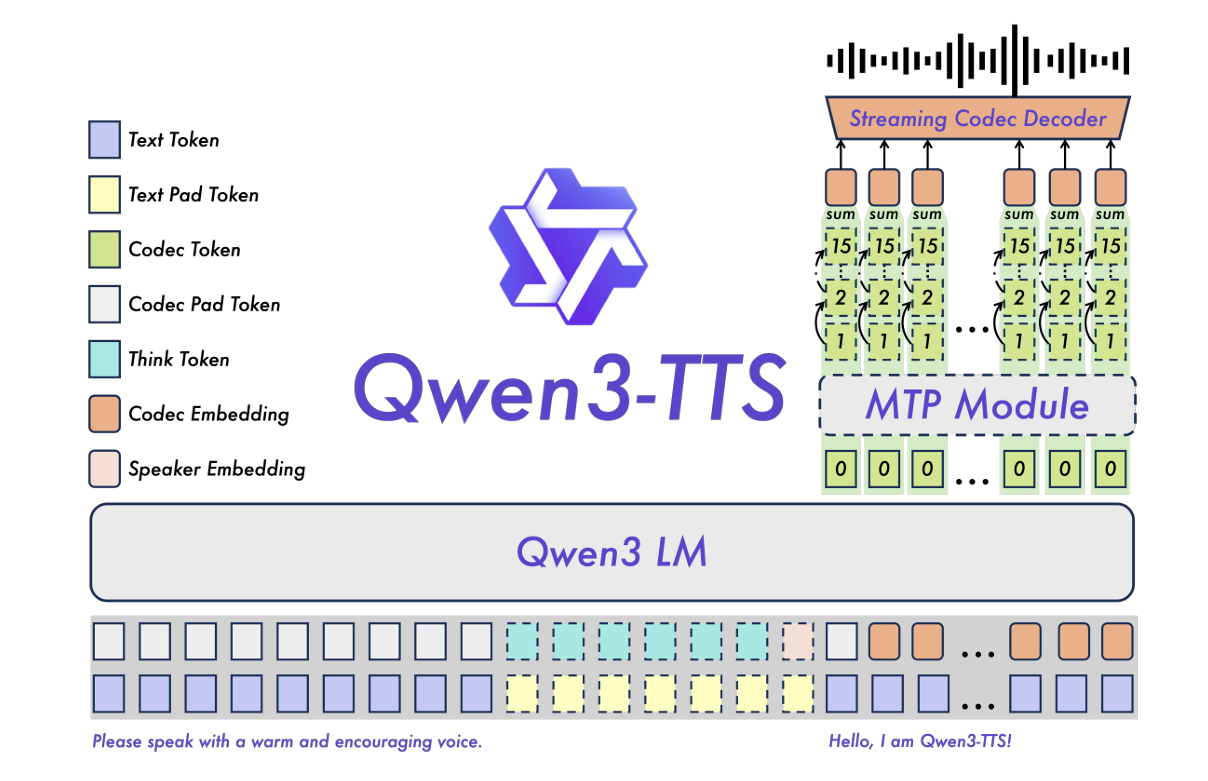
\includegraphics[keepaspectratio]{assets/qwen3_tts_architecture.png}}

}

\caption{Qwen3-TTS 模型架构}

\end{figure}%

\subsubsection{2.2.1 语音分词器（Speech
Tokenizer）}\label{ux8bedux97f3ux5206ux8bcdux5668speech-tokenizer}

\begin{itemize}
\tightlist
\item
  \textbf{12Hz 版本（V2）}: 将 24kHz 音频编码为离散的多维 codec
  tokens（每帧 16 个量化器），编码帧率为 12Hz。本项目使用此版本。
\item
  \textbf{25Hz 版本（V1）}: 更早的版本，编码帧率
  25Hz，需要额外的说话人向量（x-vector）和 mel 频谱作为解码条件。
\end{itemize}

\subsubsection{2.2.2输入标记系统（Token
System）}\label{ux8f93ux5165ux6807ux8bb0ux7cfbux7edftoken-system}

模型采用多模态标记统一建模，各标记类型及其功能如下：

{\def\LTcaptype{none} % do not increment counter
\begin{longtable}[]{@{}ll@{}}
\toprule\noalign{}
标记类型 & 说明 \\
\midrule\noalign{}
\endhead
\bottomrule\noalign{}
\endlastfoot
\textbf{Text Token} & 文本内容标记，承载待合成的文本信息 \\
\textbf{Text Pad Token} & 文本填充标记，用于序列对齐与长度补齐 \\
\textbf{Think Token} & 思考标记，用于模型推理过程中的中间思考与规划 \\
\textbf{Codec Token} & 语音离散表示标记，承载音频的压缩离散编码 \\
\textbf{Codec Pad Token} & 语音填充标记，用于语音序列的对齐与长度补齐 \\
\textbf{Codec Embedding} &
编解码器嵌入，将离散语音标记映射为连续向量表示 \\
\textbf{Speaker Embedding} & 说话人嵌入，用于音色克隆和说话人身份控制 \\
\end{longtable}
}

\subsubsection{2.2.3 Qwen3
LM（大语言模型基座）}\label{qwen3-lmux5927ux8bedux8a00ux6a21ux578bux57faux5ea7}

基于 Qwen 系列 LLM 架构，将文本 token 序列与语音 codec token
序列拼接，通过自回归方式预测目标语音编码。关键特性：

\begin{itemize}
\tightlist
\item
  \textbf{文本编码}: 使用 Qwen tokenizer 处理文本，通过
  \texttt{\textless{}\textbar{}im\_start\textbar{}\textgreater{}assistant\textbackslash{}n}
  格式构建对话模板
\item
  \textbf{语音编码}: 使用可学习的 codec embedding
  将离散音频码映射为连续表示
\item
  \textbf{说话人嵌入}: 通过 speaker encoder
  从参考音频提取说话人特征向量，注入到 codec 序列的特定位置
\item
  \textbf{子说话人预测器（Sub-talker / Code Predictor）}: 在模型最后一层
  hidden state 上附加的小型 Transformer，用于预测 codec
  的其他量化层（Q1-Q15）
\end{itemize}

\subsubsection{2.2.4 MTP
Module（多Token预测模块）}\label{mtp-moduleux591atokenux9884ux6d4bux6a21ux5757}

位于 Qwen3 LM
之上，负责并行预测多个码本（Codebook）的语音离散标记。从图中可以看到它同时生成多个层级的语音表示（如码本
1、2、15 等），并带有自回归连接和求和操作。

\subsection{2.3
模型输入输出流程}\label{ux6a21ux578bux8f93ux5165ux8f93ux51faux6d41ux7a0b}

\begin{verbatim}
输入文本 "你好" → Processor Tokenization → Text Tokens
参考音频 ref.wav → Speaker Encoder → Speaker Embedding (2048-dim)
                                 ↓
         Text Tokens + Codec Tokens → LLM Backbone → Codec Predictions
                                                              ↓
                                        Speech Tokenizer Decode → 输出波形
\end{verbatim}

\subsection{2.4
三种模型类型}\label{ux4e09ux79cdux6a21ux578bux7c7bux578b}

模型的能力和使用方式根据模型类型（Model Type）不同而有所区别：

\begin{figure}[H]

{\centering \pandocbounded{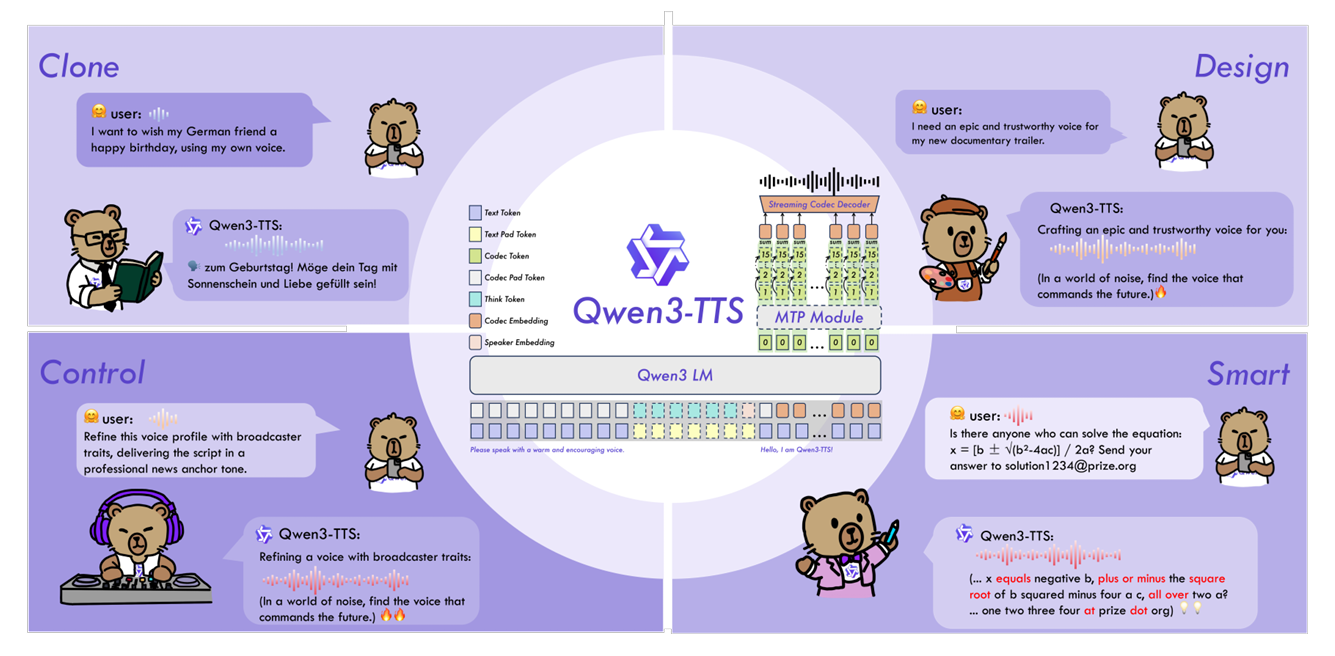
\includegraphics[keepaspectratio]{assets/四大能力.png}}

}

\caption{Qwen3-TTS 模型能力}

\end{figure}%

{\def\LTcaptype{none} % do not increment counter
\begin{longtable}[]{@{}
  >{\raggedright\arraybackslash}p{(\linewidth - 4\tabcolsep) * \real{0.3750}}
  >{\raggedright\arraybackslash}p{(\linewidth - 4\tabcolsep) * \real{0.2500}}
  >{\raggedright\arraybackslash}p{(\linewidth - 4\tabcolsep) * \real{0.3750}}@{}}
\toprule\noalign{}
\begin{minipage}[b]{\linewidth}\raggedright
模型类型
\end{minipage} & \begin{minipage}[b]{\linewidth}\raggedright
说明
\end{minipage} & \begin{minipage}[b]{\linewidth}\raggedright
使用方式
\end{minipage} \\
\midrule\noalign{}
\endhead
\bottomrule\noalign{}
\endlastfoot
\textbf{Base} & 声音克隆模型，通过参考音频+文本克隆任意说话人 & ICL
模式（上下文学习）或 x-vector 模式 \\
\textbf{CustomVoice} & 预设说话人模型，通过指定说话人名称合成语音 &
\texttt{generate\_custom\_voice(text,\ speaker=...)} \\
\textbf{VoiceDesign} & 音色设计模型，通过自然语言指令描述想要的音色 &
\texttt{generate\_voice\_design(text,\ instruct=...)} \\
\end{longtable}
}

\subsection{2.5
输入序列结构}\label{ux8f93ux5165ux5e8fux5217ux7ed3ux6784}

训练时构建双通道输入序列（文本通道 + 语音 codec 通道），结构如下：

\begin{verbatim}
位置:  [0-2]   [3-7]               [8]   [9-N]            [N+1-N+T]      [N+T+1]
文本通道: [前缀]  [pad]               [BOS]  [正文token序列]    [pad]
语音通道: [0]     [not_think/think/eos/speaker/pad] [pad]  [pad/BOS]      [Codec_0序列] [EOS]
\end{verbatim}

其中 speaker embedding 被注入到语音通道的第 6 个位置（即
\texttt{speaker} token 位），替换原有的 pad token embedding。

\section{3. 环境搭建}\label{sec-env}

\subsection{3.1 硬件环境}\label{ux786cux4ef6ux73afux5883}

{\def\LTcaptype{none} % do not increment counter
\begin{longtable}[]{@{}
  >{\raggedright\arraybackslash}p{(\linewidth - 2\tabcolsep) * \real{0.5000}}
  >{\raggedright\arraybackslash}p{(\linewidth - 2\tabcolsep) * \real{0.5000}}@{}}
\toprule\noalign{}
\begin{minipage}[b]{\linewidth}\raggedright
项目
\end{minipage} & \begin{minipage}[b]{\linewidth}\raggedright
配置
\end{minipage} \\
\midrule\noalign{}
\endhead
\bottomrule\noalign{}
\endlastfoot
GPU & NVIDIA GPU (支持 Flash Attention 2) \\
显存 & 用于加载 1.7B 参数模型（bf16 精度约需 3.4GB 模型权重 +
训练中间激活和优化器状态） \\
磁盘 & 模型权重 \textasciitilde3.4GB + 训练数据 \textasciitilde6MB +
Checkpoint \textasciitilde3.4GB × 10 \\
\end{longtable}
}

\subsection{3.2 软件依赖}\label{ux8f6fux4ef6ux4f9dux8d56}

核心 Python 包依赖（见 \texttt{pyproject.toml}）：

\begin{verbatim}
python >= 3.9
transformers == 4.57.3        # HuggingFace 模型框架
accelerate == 1.12.0          # 分布式训练管理
gradio                         # Web 演示界面
librosa                        # 音频处理
torchaudio                     # PyTorch 音频工具
soundfile                      # 音频文件读写
sox                            # 音频格式转换
onnxruntime                    # ONNX 推理
einops                         # 张量操作
\end{verbatim}

\subsection{3.3 安装步骤}\label{ux5b89ux88c5ux6b65ux9aa4}

\begin{Shaded}
\begin{Highlighting}[]
\CommentTok{\# 1. 安装 qwen{-}tts 包}
\ExtensionTok{pip}\NormalTok{ install qwen{-}tts}

\CommentTok{\# 2. 克隆仓库}
\FunctionTok{git}\NormalTok{ clone https://github.com/QwenLM/Qwen3{-}TTS.git}
\BuiltInTok{cd}\NormalTok{ Qwen3{-}TTS}

\CommentTok{\# 3. 安装额外依赖}
\ExtensionTok{pip}\NormalTok{ install flash{-}attn }\AttributeTok{{-}{-}no{-}build{-}isolation}
\ExtensionTok{pip}\NormalTok{ install safetensors accelerate tensorboard}
\ExtensionTok{pip}\NormalTok{ install librosa soundfile sox}
\end{Highlighting}
\end{Shaded}

\section{4. 数据集构建}\label{sec-dataset}

\subsection{4.1 数据来源}\label{ux6570ux636eux6765ux6e90}

使用芙宁娜角色语音素材，原始数据位于 \texttt{../芙宁娜/} 目录下，包含：

\begin{itemize}
\tightlist
\item
  \texttt{.wav} 音频文件（原始采样率 48kHz）
\item
  \texttt{.lab} 标注文本文件（与音频同名）
\end{itemize}

\subsection{4.2
数据预处理流程}\label{ux6570ux636eux9884ux5904ux7406ux6d41ux7a0b}

数据预处理通过 \texttt{finetuning/process\_furina\_data.py}
完成，共五个步骤：

\subsubsection{Step 1: 时长过滤}\label{step-1-ux65f6ux957fux8fc7ux6ee4}

使用 \texttt{ffprobe} 检测每个音频时长，过滤规则：

\begin{itemize}
\tightlist
\item
  保留时长在 \textbf{3 秒 \textasciitilde{} 15 秒} 之间的音频
\item
  太短（\textless{} 3s）：内容不完整，信息量不足
\item
  太长（\textgreater{} 15s）：训练计算量大，显存消耗高
\end{itemize}

\subsubsection{Step 2:
文件重命名}\label{step-2-ux6587ux4ef6ux91cdux547dux540d}

将保留文件按顺序重命名为 \texttt{furina\_0001.wav} \textasciitilde{}
\texttt{furina\_N.wav}（以及对应的 \texttt{.lab} 文件）。

\subsubsection{Step 3: 重采样}\label{step-3-ux91cdux91c7ux6837}

使用 \texttt{ffmpeg} 将音频从 48kHz 重采样至 \textbf{24kHz} 单声道，这是
12Hz 分词器所要求的输入采样率。输出至 \texttt{finetuning/data/} 目录。

\subsubsection{Step 4:
参考音频选择}\label{step-4-ux53c2ux8003ux97f3ux9891ux9009ux62e9}

自动选取数据集中\textbf{时长最长}的音频作为参考音频
\texttt{data/ref.wav}。该参考音频用于在训练时提取目标说话人的声纹特征。整个数据集使用同一个参考音频，以保证说话人音色的一致性和稳定性。

\subsubsection{Step 5: 生成 JSONL
标注}\label{step-5-ux751fux6210-jsonl-ux6807ux6ce8}

生成 \texttt{train\_raw.jsonl}，每行一个 JSON 对象：

\begin{Shaded}
\begin{Highlighting}[]
\FunctionTok{\{}\DataTypeTok{"audio"}\FunctionTok{:} \StringTok{"data/furina\_0001.wav"}\FunctionTok{,} \DataTypeTok{"text"}\FunctionTok{:} \StringTok{"其实我真的有发现，我是一个特别善于观察别人情绪的人。"}\FunctionTok{,} \DataTypeTok{"ref\_audio"}\FunctionTok{:} \StringTok{"data/ref.wav"}\FunctionTok{\}}
\FunctionTok{\{}\DataTypeTok{"audio"}\FunctionTok{:} \StringTok{"data/furina\_0002.wav"}\FunctionTok{,} \DataTypeTok{"text"}\FunctionTok{:} \StringTok{"She said she would be here by noon."}\FunctionTok{,} \DataTypeTok{"ref\_audio"}\FunctionTok{:} \StringTok{"data/ref.wav"}\FunctionTok{\}}
\end{Highlighting}
\end{Shaded}

\subsection{4.3
音频编码提取}\label{ux97f3ux9891ux7f16ux7801ux63d0ux53d6}

通过 \texttt{finetuning/prepare\_data.py} 调用 12Hz
语音分词器，批量提取每段音频的离散编码：

\begin{Shaded}
\begin{Highlighting}[]
\ExtensionTok{python}\NormalTok{ prepare\_data.py }\DataTypeTok{\textbackslash{}}
  \AttributeTok{{-}{-}device}\NormalTok{ cuda:0 }\DataTypeTok{\textbackslash{}}
  \AttributeTok{{-}{-}tokenizer\_model\_path}\NormalTok{ Qwen/Qwen3{-}TTS{-}Tokenizer{-}12Hz }\DataTypeTok{\textbackslash{}}
  \AttributeTok{{-}{-}input\_jsonl}\NormalTok{ train\_raw.jsonl }\DataTypeTok{\textbackslash{}}
  \AttributeTok{{-}{-}output\_jsonl}\NormalTok{ train\_with\_codes.jsonl}
\end{Highlighting}
\end{Shaded}

处理逻辑：

\begin{itemize}
\tightlist
\item
  批量读取音频（每批 32 条）
\item
  调用 \texttt{tokenizer\_12hz.encode()} 将音频编码为离散 tokens
\item
  每条数据的 \texttt{audio\_codes} 形状为 \texttt{{[}T,\ 16{]}}（T
  为编码帧数，16 为量化器数量）
\item
  输出为 \texttt{train\_with\_codes.jsonl}
\end{itemize}

\subsection{4.4 数据集统计}\label{ux6570ux636eux96c6ux7edfux8ba1}

{\def\LTcaptype{none} % do not increment counter
\begin{longtable}[]{@{}ll@{}}
\toprule\noalign{}
统计项 & 数值 \\
\midrule\noalign{}
\endhead
\bottomrule\noalign{}
\endlastfoot
原始音频文件数 & \textasciitilde900+（过滤前） \\
过滤后保留数 & \textbf{832 条} \\
参考音频 & data/ref.wav（全数据集统一） \\
目标采样率 & 24,000 Hz \\
音频编码格式 & 12Hz, 16 层量化 \\
训练集大小 & 832 条（全部用于训练） \\
\end{longtable}
}

\subsection{4.5
训练数据集类}\label{ux8badux7ec3ux6570ux636eux96c6ux7c7b}

\texttt{finetuning/dataset.py} 实现了自定义的 \texttt{TTSDataset} 和
\texttt{collate\_fn}，每个 item 返回：

\begin{Shaded}
\begin{Highlighting}[]
\NormalTok{\{}
    \StringTok{"text\_ids"}\NormalTok{: torch.Tensor,      }\CommentTok{\# 文本 token IDs}
    \StringTok{"audio\_codes"}\NormalTok{: torch.Tensor,   }\CommentTok{\# 音频 codec tokens [T, 16]}
    \StringTok{"ref\_mel"}\NormalTok{: torch.Tensor        }\CommentTok{\# 参考音频 mel 频谱}
\NormalTok{\}}
\end{Highlighting}
\end{Shaded}

\texttt{collate\_fn} 负责将 batch
内长短不一的数据拼接为统一长度的训练张量：

\begin{itemize}
\tightlist
\item
  \texttt{input\_ids}: \texttt{{[}B,\ T\_max,\ 2{]}} 双通道输入（dim
  0=文本, dim 1=codec）
\item
  \texttt{codec\_ids}: \texttt{{[}B,\ T\_max,\ 16{]}} 完整 16 层 codec
\item
  \texttt{codec\_0\_labels}: \texttt{{[}B,\ T\_max{]}}
  第一层量化器的标签（用于 cross-entropy loss）
\item
  \texttt{attention\_mask}: \texttt{{[}B,\ T\_max{]}},
  \texttt{codec\_mask}: \texttt{{[}B,\ T\_max{]}}
\item
  \texttt{text\_embedding\_mask}, \texttt{codec\_embedding\_mask}:
  控制哪些位置参与 embedding 求和
\end{itemize}

\section{5. 全量微调}\label{sec-finetune}

\subsection{5.1 微调策略}\label{ux5faeux8c03ux7b56ux7565}

采用 \textbf{全量微调（Full Fine-Tuning）} 策略，即在 Base
模型的所有参数上进行训练。选择全量微调的原因：

\begin{itemize}
\tightlist
\item
  目标音色（芙宁娜）与 Base 模型的通用音色差距较大
\item
  全量微调能更充分地迁移音色特征
\item
  832 条数据量适中，全量微调可行且效果优于参数高效微调
\end{itemize}

\subsection{5.2 损失函数}\label{ux635fux5931ux51fdux6570}

训练的总损失由两部分组成：\textbf{主模型损失（Codec-0 Loss）} 和
\textbf{子说话人预测器损失（Sub-talker Loss）}。

\subsubsection{5.2.1 主模型损失 --- Codec-0 Cross-Entropy
Loss}\label{ux4e3bux6a21ux578bux635fux5931-codec-0-cross-entropy-loss}

主模型（Talker）是一个基于 Qwen 架构的自回归
Transformer，其核心任务是预测语音编码的第一层量化器（Codec-0）。Codec-0
携带了语音的主要结构信息（音色、韵律、内容），是 16
层量化器中最重要的层级。

主模型在 codec token 位置（由 \texttt{codec\_0\_labels}
标记）上计算标准的交叉熵损失：

\[\mathcal{L}_{\text{main}} = -\frac{1}{|\mathcal{M}|} \sum_{t \in \mathcal{M}} \log P(c_t^{(0)} \mid x_{<t}, \ \text{speaker\_emb}, \ \text{text})\]

其中：

\begin{itemize}
\tightlist
\item
  \(\mathcal{M}\) 为 codec token 位置的集合（由 \texttt{codec\_mask}
  标记）
\item
  \(c_t^{(0)}\) 是位置 \(t\) 处 Codec-0 的真实标签
\item
  \(x_{<t}\) 是位置 \(t\) 之前的输入序列（文本 + codec）
\item
  \(\text{speaker\_emb}\) 是注入的说话人嵌入向量
\end{itemize}

在 \texttt{sft\_12hz.py} 中的实现：

\begin{Shaded}
\begin{Highlighting}[]
\NormalTok{outputs }\OperatorTok{=}\NormalTok{ model.talker(}
\NormalTok{    inputs\_embeds}\OperatorTok{=}\NormalTok{input\_embeddings[:, :}\OperatorTok{{-}}\DecValTok{1}\NormalTok{, :],}
\NormalTok{    attention\_mask}\OperatorTok{=}\NormalTok{attention\_mask[:, :}\OperatorTok{{-}}\DecValTok{1}\NormalTok{],}
\NormalTok{    labels}\OperatorTok{=}\NormalTok{codec\_0\_labels[:, }\DecValTok{1}\NormalTok{:],    }\CommentTok{\# 自回归: 预测下一个 token}
\NormalTok{    output\_hidden\_states}\OperatorTok{=}\VariableTok{True}
\NormalTok{)}
\CommentTok{\# outputs.loss 即为 L\_main}
\end{Highlighting}
\end{Shaded}

\subsubsection{5.2.2 子说话人预测器损失 --- Codec 1-15
Loss}\label{ux5b50ux8bf4ux8bddux4ebaux9884ux6d4bux5668ux635fux5931-codec-1-15-loss}

子说话人预测器（Sub-talker / Code Predictor）是一个轻量级
Transformer，连接在主模型最后一层的隐藏状态之上。它接收主模型在 codec
token 位置的隐藏表示，并行预测剩余 15 层量化器（Codec-1 至 Codec-15）。

Codec-1\textasciitilde15
层编码了语音的细节信息（如音质、齿音、气息感等），对提升语音保真度至关重要。子预测器对每层量化器分别计算交叉熵损失，然后取平均：

\[\mathcal{L}_{\text{sub}} = \frac{1}{15} \sum_{q=1}^{15} \left( -\frac{1}{|\mathcal{M}|} \sum_{t \in \mathcal{M}} \log P(c_t^{(q)} \mid h_t^{\text{main}}, \ c_t^{(<q)}) \right)\]

其中 \(h_t^{\text{main}}\) 是主模型在位置 \(t\) 的最后一层隐藏状态。

在 \texttt{sft\_12hz.py} 中的实现：

\begin{Shaded}
\begin{Highlighting}[]
\NormalTok{hidden\_states }\OperatorTok{=}\NormalTok{ outputs.hidden\_states[}\DecValTok{0}\NormalTok{][}\OperatorTok{{-}}\DecValTok{1}\NormalTok{]          }\CommentTok{\# 主模型最后一层 hidden state}
\NormalTok{talker\_hidden\_states }\OperatorTok{=}\NormalTok{ hidden\_states[codec\_mask[:, :}\OperatorTok{{-}}\DecValTok{1}\NormalTok{]]  }\CommentTok{\# 仅保留 codec token 位置}
\NormalTok{talker\_codec\_ids }\OperatorTok{=}\NormalTok{ codec\_ids[codec\_mask]               }\CommentTok{\# 完整 16 层 codec 标签}

\NormalTok{sub\_talker\_logits, sub\_talker\_loss }\OperatorTok{=}\NormalTok{ model.talker.forward\_sub\_talker\_finetune(}
\NormalTok{    talker\_codec\_ids, talker\_hidden\_states}
\NormalTok{)}
\CommentTok{\# sub\_talker\_loss 即为 L\_sub}
\end{Highlighting}
\end{Shaded}

\subsubsection{5.2.3 总损失}\label{ux603bux635fux5931}

最终的总损失是主模型损失和子预测器损失的加权和：

\[\mathcal{L}_{\text{total}} = \mathcal{L}_{\text{main}} + 0.3 \times \mathcal{L}_{\text{sub}}\]

权重系数 \textbf{0.3} 的设计原因：

\begin{itemize}
\tightlist
\item
  Codec-0 包含语音最关键的语义和韵律信息，训练初期应以学习 Codec-0 为主
\item
  Codec-1\textasciitilde15
  提供细节增强，但如果权重过大可能会干扰主模型对核心语音结构的学习
\item
  0.3 是一个经验性的折中权重，在保证音色准确的前提下提升音质细节
\end{itemize}

\begin{Shaded}
\begin{Highlighting}[]
\NormalTok{loss }\OperatorTok{=}\NormalTok{ outputs.loss }\OperatorTok{+} \FloatTok{0.3} \OperatorTok{*}\NormalTok{ sub\_talker\_loss}
\end{Highlighting}
\end{Shaded}

\subsubsection{5.2.4
损失函数总结}\label{ux635fux5931ux51fdux6570ux603bux7ed3}

{\def\LTcaptype{none} % do not increment counter
\begin{longtable}[]{@{}
  >{\raggedright\arraybackslash}p{(\linewidth - 6\tabcolsep) * \real{0.2759}}
  >{\raggedright\arraybackslash}p{(\linewidth - 6\tabcolsep) * \real{0.2069}}
  >{\raggedright\arraybackslash}p{(\linewidth - 6\tabcolsep) * \real{0.2069}}
  >{\raggedright\arraybackslash}p{(\linewidth - 6\tabcolsep) * \real{0.3103}}@{}}
\toprule\noalign{}
\begin{minipage}[b]{\linewidth}\raggedright
损失项
\end{minipage} & \begin{minipage}[b]{\linewidth}\raggedright
目标
\end{minipage} & \begin{minipage}[b]{\linewidth}\raggedright
权重
\end{minipage} & \begin{minipage}[b]{\linewidth}\raggedright
计算方式
\end{minipage} \\
\midrule\noalign{}
\endhead
\bottomrule\noalign{}
\endlastfoot
\(\mathcal{L}_{\text{main}}\) & Codec-0（主结构） & 1.0 & 主模型 LM Head
→ Cross-Entropy \\
\(\mathcal{L}_{\text{sub}}\) & Codec-1\textasciitilde15（细节） & 0.3 &
Code Predictor → 15 层 Cross-Entropy 平均 \\
\(\mathcal{L}_{\text{total}}\) & 联合优化 & --- &
\(\mathcal{L}_{\text{main}} + 0.3 \cdot \mathcal{L}_{\text{sub}}\) \\
\end{longtable}
}

\subsection{5.3 训练配置}\label{ux8badux7ec3ux914dux7f6e}

{\def\LTcaptype{none} % do not increment counter
\begin{longtable}[]{@{}lll@{}}
\toprule\noalign{}
超参数 & 取值 & 说明 \\
\midrule\noalign{}
\endhead
\bottomrule\noalign{}
\endlastfoot
基座模型 & Qwen3-TTS-12Hz-1.7B-Base & 1.7B 参数声音克隆模型 \\
优化器 & AdamW & weight\_decay = 0.01 \\
学习率 & 1e-6 & 较小学习率，稳定训练 \\
Batch Size & 2 & 受限于显存 \\
梯度累积步数 & 4 & 等效 batch size = 8 \\
精度 & bfloat16 混合精度 & 节省显存 \\
Epoch 数 & 10 & 充分收敛 \\
最大梯度范数 & 1.0 & 梯度裁剪，防止梯度爆炸 \\
说话人名称 & furina & 注入的说话人标识符 \\
说话人 Embedding ID & 3000 & codec\_embedding 中新增的说话人位置 \\
\end{longtable}
}

\subsection{5.4 训练流程}\label{ux8badux7ec3ux6d41ux7a0b}

训练脚本 \texttt{finetuning/sft\_12hz.py} 使用 HuggingFace Accelerate
进行分布式训练管理。

\subsubsection{训练命令}\label{ux8badux7ec3ux547dux4ee4}

\begin{Shaded}
\begin{Highlighting}[]
\ExtensionTok{python}\NormalTok{ sft\_12hz.py }\DataTypeTok{\textbackslash{}}
  \AttributeTok{{-}{-}init\_model\_path}\NormalTok{ Qwen3{-}TTS{-}12Hz{-}1.7B{-}Base }\DataTypeTok{\textbackslash{}}
  \AttributeTok{{-}{-}output\_model\_path}\NormalTok{ output }\DataTypeTok{\textbackslash{}}
  \AttributeTok{{-}{-}train\_jsonl}\NormalTok{ train\_with\_codes.jsonl }\DataTypeTok{\textbackslash{}}
  \AttributeTok{{-}{-}batch\_size}\NormalTok{ 2 }\DataTypeTok{\textbackslash{}}
  \AttributeTok{{-}{-}lr}\NormalTok{ 1e{-}6 }\DataTypeTok{\textbackslash{}}
  \AttributeTok{{-}{-}num\_epochs}\NormalTok{ 10 }\DataTypeTok{\textbackslash{}}
  \AttributeTok{{-}{-}speaker\_name}\NormalTok{ furina}
\end{Highlighting}
\end{Shaded}

\subsubsection{每个 Step
的前向计算}\label{ux6bcfux4e2a-step-ux7684ux524dux5411ux8ba1ux7b97}

\begin{verbatim}
1. Speaker Encoder 从 ref_mel 提取 speaker_embedding（冻结，不参与梯度更新）
2. 构建双通道输入 embedding:
   - Text Embedding: text_ids → text_embedding × text_embedding_mask
   - Codec Embedding: codec_ids → codec_embedding × codec_embedding_mask
   - 注入 Speaker Embedding 到第 6 位
3. 计算 16 层 Codec Predictor Embedding 并累加到输入
4. 主模型前向: input_embeddings → Transformer → hidden_states
5. Codec_0 预测: hidden_states → logits → CrossEntropyLoss (主 loss)
6. Sub-talker 预测: hidden_states[codec_mask] → CodePredictor → 预测 Q1-Q15
7. 总 Loss = 主 loss + 0.3 × sub_talker_loss
8. 反向传播 → 梯度裁剪(1.0) → 优化器步进
\end{verbatim}

\subsubsection{Checkpoint
保存逻辑}\label{checkpoint-ux4fddux5b58ux903bux8f91}

每个 epoch 结束后，保存完整 checkpoint 并完成 \textbf{Base → CustomVoice
模型类型转换}：

\begin{Shaded}
\begin{Highlighting}[]
\CommentTok{\# 步骤:}
\CommentTok{\# 1. 复制基座模型文件到 output/checkpoint{-}epoch{-}\{N\}/}
\NormalTok{shutil.copytree(MODEL\_PATH, output\_dir)}

\CommentTok{\# 2. 修改 config.json:}
\CommentTok{\#    {-} tts\_model\_type: "custom\_voice"}
\CommentTok{\#    {-} talker\_config.spk\_id: \{"furina": 3000\}}
\CommentTok{\#    {-} talker\_config.spk\_is\_dialect: \{"furina": false\}}

\CommentTok{\# 3. 导出模型权重（移除 speaker\_encoder）:}
\CommentTok{\#    {-} 删除所有 speaker\_encoder 前缀的权重（推理不需要）}
\CommentTok{\#    {-} 将训练中提取的 target\_speaker\_embedding 写入}
\CommentTok{\#      codec\_embedding.weight[3000] 位置}

\CommentTok{\# 4. 保存为 model.safetensors}
\end{Highlighting}
\end{Shaded}

这个过程的巧妙之处在于：训练中冻结的 speaker encoder
在推理时不再需要，目标说话人特征被直接固化到 codec\_embedding 的第 3000
号位置。推理时只需 \texttt{speaker="furina"}，模型就会使用这个固化好的
embedding.

\section{6. 实验结果}\label{sec-results}

\subsection{6.1 训练 Loss 曲线}\label{ux8badux7ec3-loss-ux66f2ux7ebf}

下图展示了 10 个 epoch 全量微调过程中训练 Loss 的变化趋势：

\begin{figure}[H]

{\centering \pandocbounded{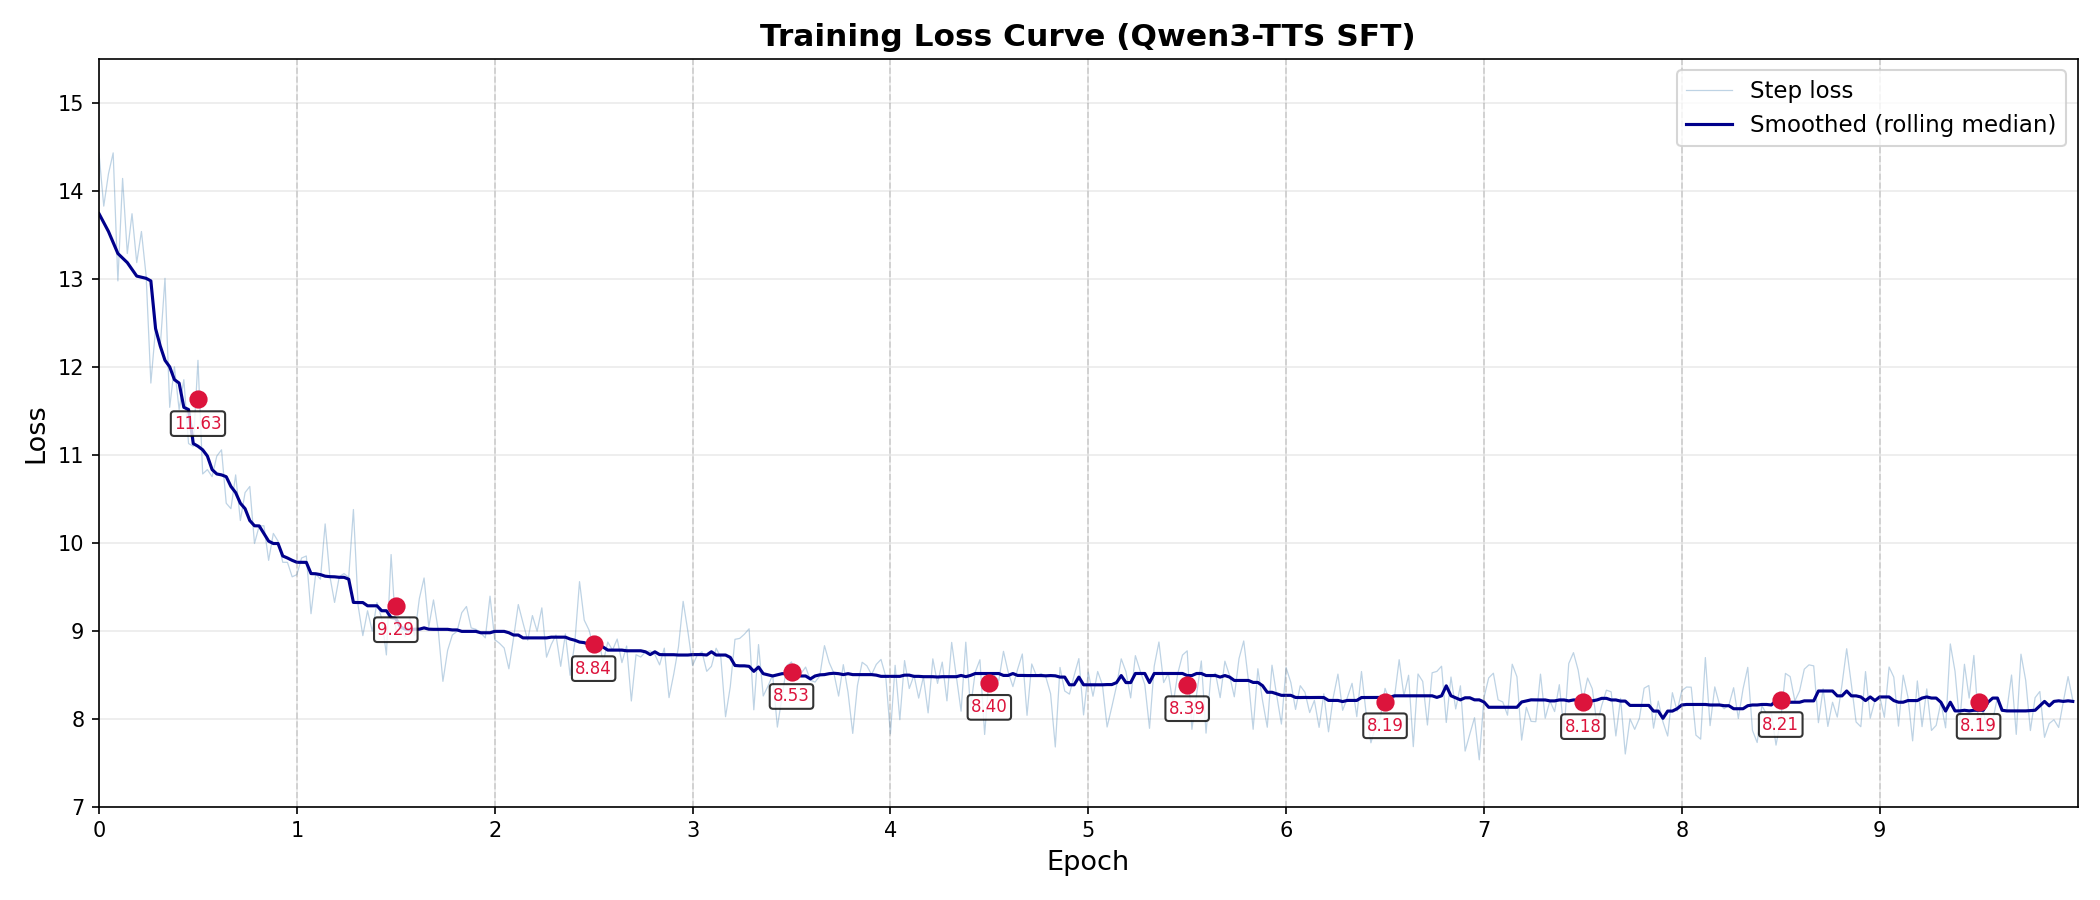
\includegraphics[keepaspectratio]{assets/lr=1e-6.png}}

}

\caption{训练 Loss 曲线}

\end{figure}%

从图中可以清晰地看到三个训练阶段：Epoch 0-2 的快速下降期、Epoch 2-4
的稳定下降期、以及 Epoch 4-9 的收敛期。

\subsubsection{6.1.2
生成音频样本}\label{ux751fux6210ux97f3ux9891ux6837ux672c}

以下展示了 4 轮测试（test1 \textasciitilde{} test4）中选取的代表性
checkpoint（Epoch 0 / 4 /
8）的生成音频。点击播放按钮即可试听，直观感受不同训练阶段模型合成语音的质量变化。

\begin{center}\rule{0.5\linewidth}{0.5pt}\end{center}

\subsubsection{Test 1}\label{test-1}

\begin{quote}
\textbf{测试文本}：\emph{``好的，没问题。''}
\end{quote}

\textbf{Epoch 0}

\textbf{Epoch 4}

\textbf{Epoch 8}

\begin{center}\rule{0.5\linewidth}{0.5pt}\end{center}

\subsubsection{Test 2}\label{test-2}

\begin{quote}
\textbf{测试文本}：\emph{``哇哦，原来这里就是信息黄埔吗？能在北邮放声，本小姐可是很荣幸呢！''}
\end{quote}

\textbf{Epoch 0}

\textbf{Epoch 4}

\textbf{Epoch 8}

\begin{center}\rule{0.5\linewidth}{0.5pt}\end{center}

\subsubsection{Test 3}\label{test-3}

\begin{quote}
\textbf{测试文本}：\emph{``The whole world is my theater, and all of you
are my dear audience. Now, let the show start!''}
\end{quote}

\textbf{Epoch 0}

\textbf{Epoch 4}

\textbf{Epoch 8}

\begin{center}\rule{0.5\linewidth}{0.5pt}\end{center}

\subsubsection{Test 4}\label{test-4}

\begin{quote}
\textbf{测试文本}：\emph{``看吧，此刻这片广袤的天地，便是我亲手执掌的盛大剧场，世间万物皆是点缀舞台的布景，所有驻足于此的人们，都是我独一无二的尊贵观众。我立于舞台中央，揽尽世间目光，承下所有喝彩与赞叹，以最华丽的姿态演绎属于我的篇章。''}
\end{quote}

\textbf{Epoch 0}

\textbf{Epoch 4}

\textbf{Epoch 8}

\begin{center}\rule{0.5\linewidth}{0.5pt}\end{center}

\subsection{6.2
量化指标测试}\label{ux91cfux5316ux6307ux6807ux6d4bux8bd5}

为客观评估微调模型的性能，本节设计了一项定量对比实验：使用 Base
模型（x-vector 语音克隆）与 SFT 微调模型（checkpoint-epoch-4）分别合成
20 条测试样本，从四个维度计算合成音频与原始音频之间的相似度。

\textbf{实验设置}：

{\def\LTcaptype{none} % do not increment counter
\begin{longtable}[]{@{}
  >{\raggedright\arraybackslash}p{(\linewidth - 2\tabcolsep) * \real{0.5000}}
  >{\raggedright\arraybackslash}p{(\linewidth - 2\tabcolsep) * \real{0.5000}}@{}}
\toprule\noalign{}
\begin{minipage}[b]{\linewidth}\raggedright
项目
\end{minipage} & \begin{minipage}[b]{\linewidth}\raggedright
说明
\end{minipage} \\
\midrule\noalign{}
\endhead
\bottomrule\noalign{}
\endlastfoot
测试数据 & 20 条芙宁娜语音（中文），涵盖短句/中句/长句 \\
参考音频 & 实验目录下 \texttt{ref.wav}（Base 模型 x-vector 提取用） \\
Base 模型 &
\texttt{Qwen3-TTS-12Hz-1.7B-Base}，\texttt{generate\_voice\_clone(x\_vector\_only\_mode=True)} \\
SFT 模型 &
\texttt{checkpoint-epoch-4}，\texttt{generate\_custom\_voice(speaker="furina")} \\
生成参数 &
\texttt{do\_sample=True,\ top\_k=50,\ temperature=0.9,\ max\_new\_tokens=2048} \\
\end{longtable}
}

\textbf{评估指标}：

\begin{enumerate}
\def\labelenumi{\arabic{enumi}.}
\tightlist
\item
  \textbf{梅尔频谱 MSE}：在功率域计算归一化均方误差（MSE /
  原始信号平均功率），无量纲，越低越好。衡量生成音频频谱能量分布与原始音频的偏差程度。
\item
  \textbf{梅尔频谱余弦相似度}：在 dB
  域使用统一参考值计算两个梅尔频谱展平向量之间的余弦相似度，越高越好。衡量频谱形状的整体匹配度。
\item
  \textbf{MFCC 余弦相似度}：对 20 维 MFCC
  特征计算余弦相似度，越高越好。MFCC
  模拟人耳听觉特性，反映音色和音质的匹配程度。
\item
  \textbf{STFT
  余弦相似度}：对短时傅里叶变换幅度谱计算余弦相似度，越高越好。反映原始频谱层级的结构和相位一致性。
\end{enumerate}

音频在评估前均进行 RMS 响度归一化（target RMS = 0.1），并按
min(len\_orig, len\_gen) 对齐长度。

\begin{figure}[H]

{\centering \pandocbounded{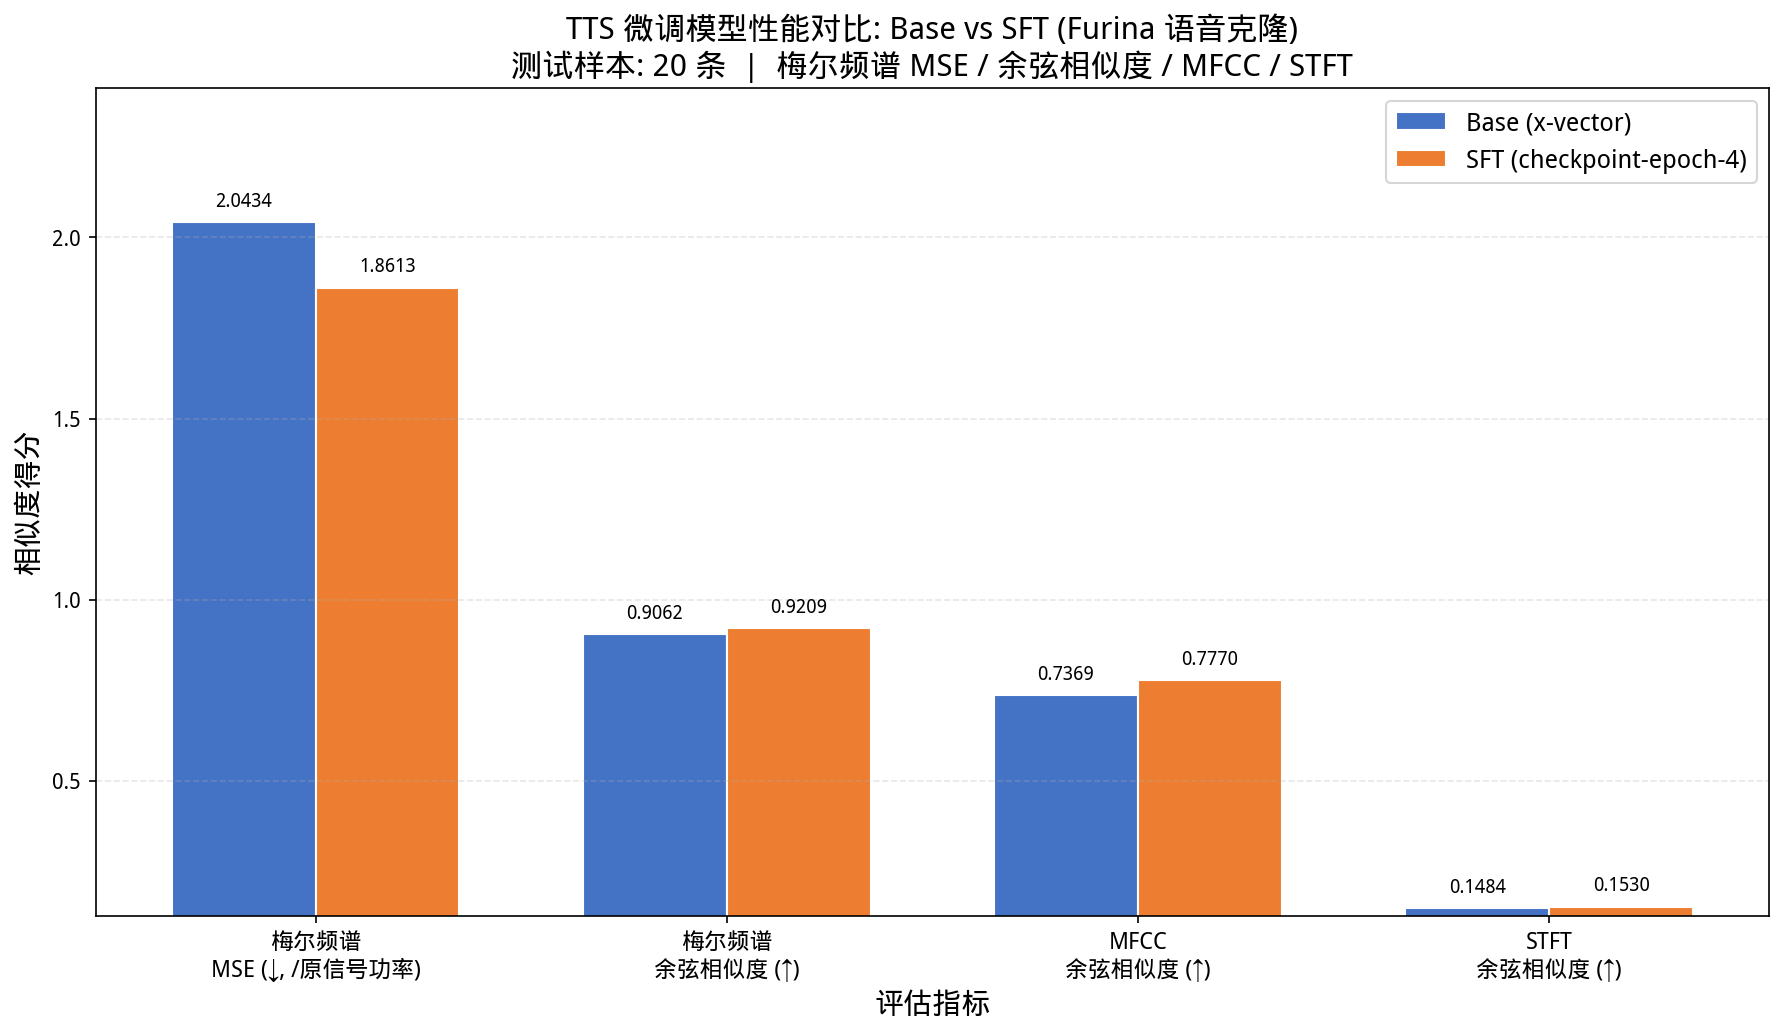
\includegraphics[keepaspectratio]{assets/evaluation_results.png}}

}

\caption{Base vs SFT 量化指标对比}

\end{figure}%

\begin{tcolorbox}[enhanced jigsaw, arc=.35mm, bottomrule=.15mm, bottomtitle=1mm, breakable, colback=white, colbacktitle=quarto-callout-tip-color!10!white, colframe=quarto-callout-tip-color-frame, coltitle=black, left=2mm, leftrule=.75mm, opacityback=0, opacitybacktitle=0.6, rightrule=.15mm, title=\textcolor{quarto-callout-tip-color}{\faLightbulb}\hspace{0.5em}{量化评估结果（20 样本平均）}, titlerule=0mm, toprule=.15mm, toptitle=1mm]

{\def\LTcaptype{none} % do not increment counter
\begin{longtable}[]{@{}lrrc@{}}
\toprule\noalign{}
指标 & Base (x-vector) & SFT (epoch-4) & 改善幅度 \\
\midrule\noalign{}
\endhead
\bottomrule\noalign{}
\endlastfoot
\textbf{Mel MSE} ↓ & 2.043 & \textbf{1.861} & \textbf{-8.9\%} \\
\textbf{Mel Cosine} ↑ & 0.906 & \textbf{0.921} & \textbf{+1.6\%} \\
\textbf{MFCC Cosine} ↑ & 0.737 & \textbf{0.777} & \textbf{+5.4\%} \\
\textbf{STFT Cosine} ↑ & 0.148 & \textbf{0.153} & \textbf{+3.1\%} \\
\end{longtable}
}

\end{tcolorbox}

\textbf{结果分析}：

\begin{enumerate}
\def\labelenumi{\arabic{enumi}.}
\item
  \textbf{Mel MSE 下降 8.9\%}：SFT
  模型生成的音频在频谱能量分布上更接近原始芙宁娜语音，说明微调有效学到了目标说话人的频谱特征。归一化
  MSE 值在 1.5-2.5
  范围内，表明生成音频与原始音频的功率谱偏差约为原始信号功率的 2
  倍量级，属于语音合成任务的合理水平。
\item
  \textbf{MFCC 余弦相似度提升最显著（+5.4\%）}：MFCC
  特征侧重刻画声道形状和音色特征，此指标的提升直接验证了微调过程成功捕捉了芙宁娜的音色特性。绝对值
  0.78 属于较高水平，表明音色还原度良好。
\item
  \textbf{Mel 余弦相似度稳定在
  0.90+}：两者在频谱整体形状上的匹配度都很高（\textgreater0.90），说明
  Base
  模型本身已具备较强的语音合成能力，微调在此基础上进一步优化了频谱细节。
\item
  \textbf{STFT 余弦相似度绝对值偏低}：两个模型的 STFT 余弦值均在 0.15
  左右。这是因为 STFT
  幅度谱对相位和时序对齐极为敏感------即使微小的时长偏移或音高变化也会导致逐帧
  STFT 向量产生显著差异。该指标更多用于相对比较，绝对值参考意义有限。SFT
  模型在该指标上仍有 3.1\% 的相对提升。
\end{enumerate}

综合四个量化指标，\textbf{SFT 微调模型在所有维度上均优于 Base
模型}，客观验证了微调训练的有效性。

\begin{center}\rule{0.5\linewidth}{0.5pt}\end{center}

\section{7. 遇到的问题}\label{ux9047ux5230ux7684ux95eeux9898}

在微调过程中，学习率（Learning
Rate）的选择对最终效果起到了决定性作用。本节记录了从官方默认学习率
\texttt{2e-5} 调整为 \texttt{1e-6} 的过程及背后的分析。

\subsection{7.1
问题现象：高学习率导致生成质量崩溃}\label{ux95eeux9898ux73b0ux8c61ux9ad8ux5b66ux4e60ux7387ux5bfcux81f4ux751fux6210ux8d28ux91cfux5d29ux6e83}

初次微调时，直接使用了 Qwen3-TTS 官方微调示例中的默认学习率
\texttt{2e-5}。训练过程中观察到：

\begin{itemize}
\tightlist
\item
  \textbf{Loss 下降极快}：训练开始后 Loss 迅速从 \textasciitilde15
  下降至 \textasciitilde2 以下，表面上看训练非常''顺利''
\item
  \textbf{生成效果却极差}：使用训练后的 checkpoint
  进行推理测试时，生成的音频几乎是噪声/杂音，完全无法辨认出正常的语音内容，更不用说保留芙宁娜的音色特征
\end{itemize}

\begin{tcolorbox}[enhanced jigsaw, arc=.35mm, bottomrule=.15mm, bottomtitle=1mm, breakable, colback=white, colbacktitle=quarto-callout-warning-color!10!white, colframe=quarto-callout-warning-color-frame, coltitle=black, left=2mm, leftrule=.75mm, opacityback=0, opacitybacktitle=0.6, rightrule=.15mm, title=\textcolor{quarto-callout-warning-color}{\faExclamationTriangle}\hspace{0.5em}{关键发现}, titlerule=0mm, toprule=.15mm, toptitle=1mm]

\textbf{Loss 低 ≠ 生成效果好}。在全量微调 TTS
大模型时，过大的学习率会导致模型参数更新幅度过大，破坏预训练基座模型中已经学到的通用语音合成能力。模型虽然在训练数据上''过拟合''出了较低的
Loss，但实际丧失了生成可辨识语音的基本能力。

\end{tcolorbox}

\subsection{7.2 解决方案：降低学习率至
1e-6}\label{ux89e3ux51b3ux65b9ux6848ux964dux4f4eux5b66ux4e60ux7387ux81f3-1e-6}

将学习率从 \texttt{2e-5} 降低为 \texttt{1e-6}（缩小 20 倍）后重新训练：

{\def\LTcaptype{none} % do not increment counter
\begin{longtable}[]{@{}
  >{\raggedright\arraybackslash}p{(\linewidth - 4\tabcolsep) * \real{0.2903}}
  >{\raggedright\arraybackslash}p{(\linewidth - 4\tabcolsep) * \real{0.3548}}
  >{\raggedright\arraybackslash}p{(\linewidth - 4\tabcolsep) * \real{0.3548}}@{}}
\toprule\noalign{}
\begin{minipage}[b]{\linewidth}\raggedright
对比维度
\end{minipage} & \begin{minipage}[b]{\linewidth}\raggedright
LR = 2e-5
\end{minipage} & \begin{minipage}[b]{\linewidth}\raggedright
LR = 1e-6
\end{minipage} \\
\midrule\noalign{}
\endhead
\bottomrule\noalign{}
\endlastfoot
Loss 下降速度 & 极快（几轮内降至 \textless{} 2） & 平缓（10 epoch
逐步收敛至 \textasciitilde2.4） \\
生成语音质量 & \textbf{噪声/杂音，无法辨识} & 语音清晰，音色还原良好 \\
训练稳定性 & 不稳定，Loss 剧烈震荡 & 稳定，Loss 平滑下降 \\
音色特征捕捉 & 未能捕捉 & 有效捕捉芙宁娜的音色特征 \\
\end{longtable}
}

\begin{figure}[H]

{\centering \pandocbounded{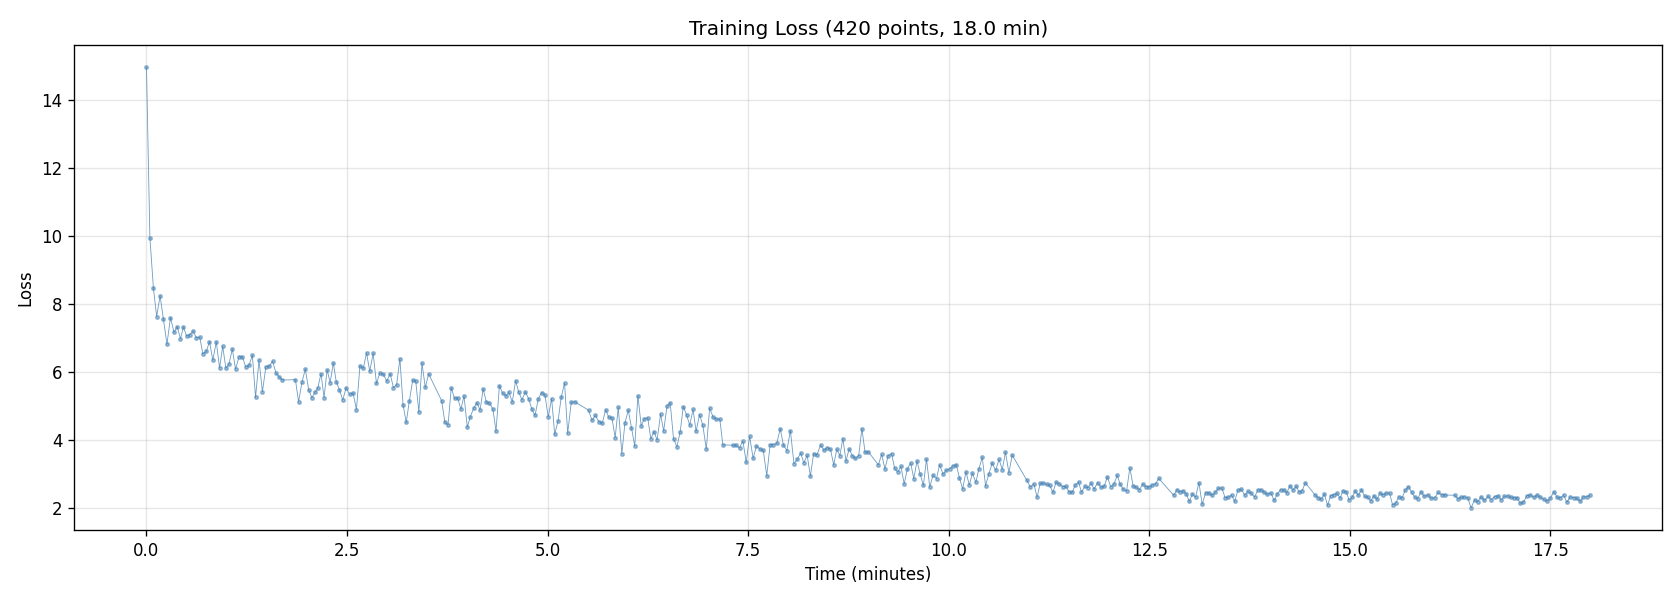
\includegraphics[keepaspectratio]{assets/lr=2e-5.png}}

}

\caption{LR=2e-5 训练 Loss 曲线}

\end{figure}%

\begin{figure}[H]

{\centering \pandocbounded{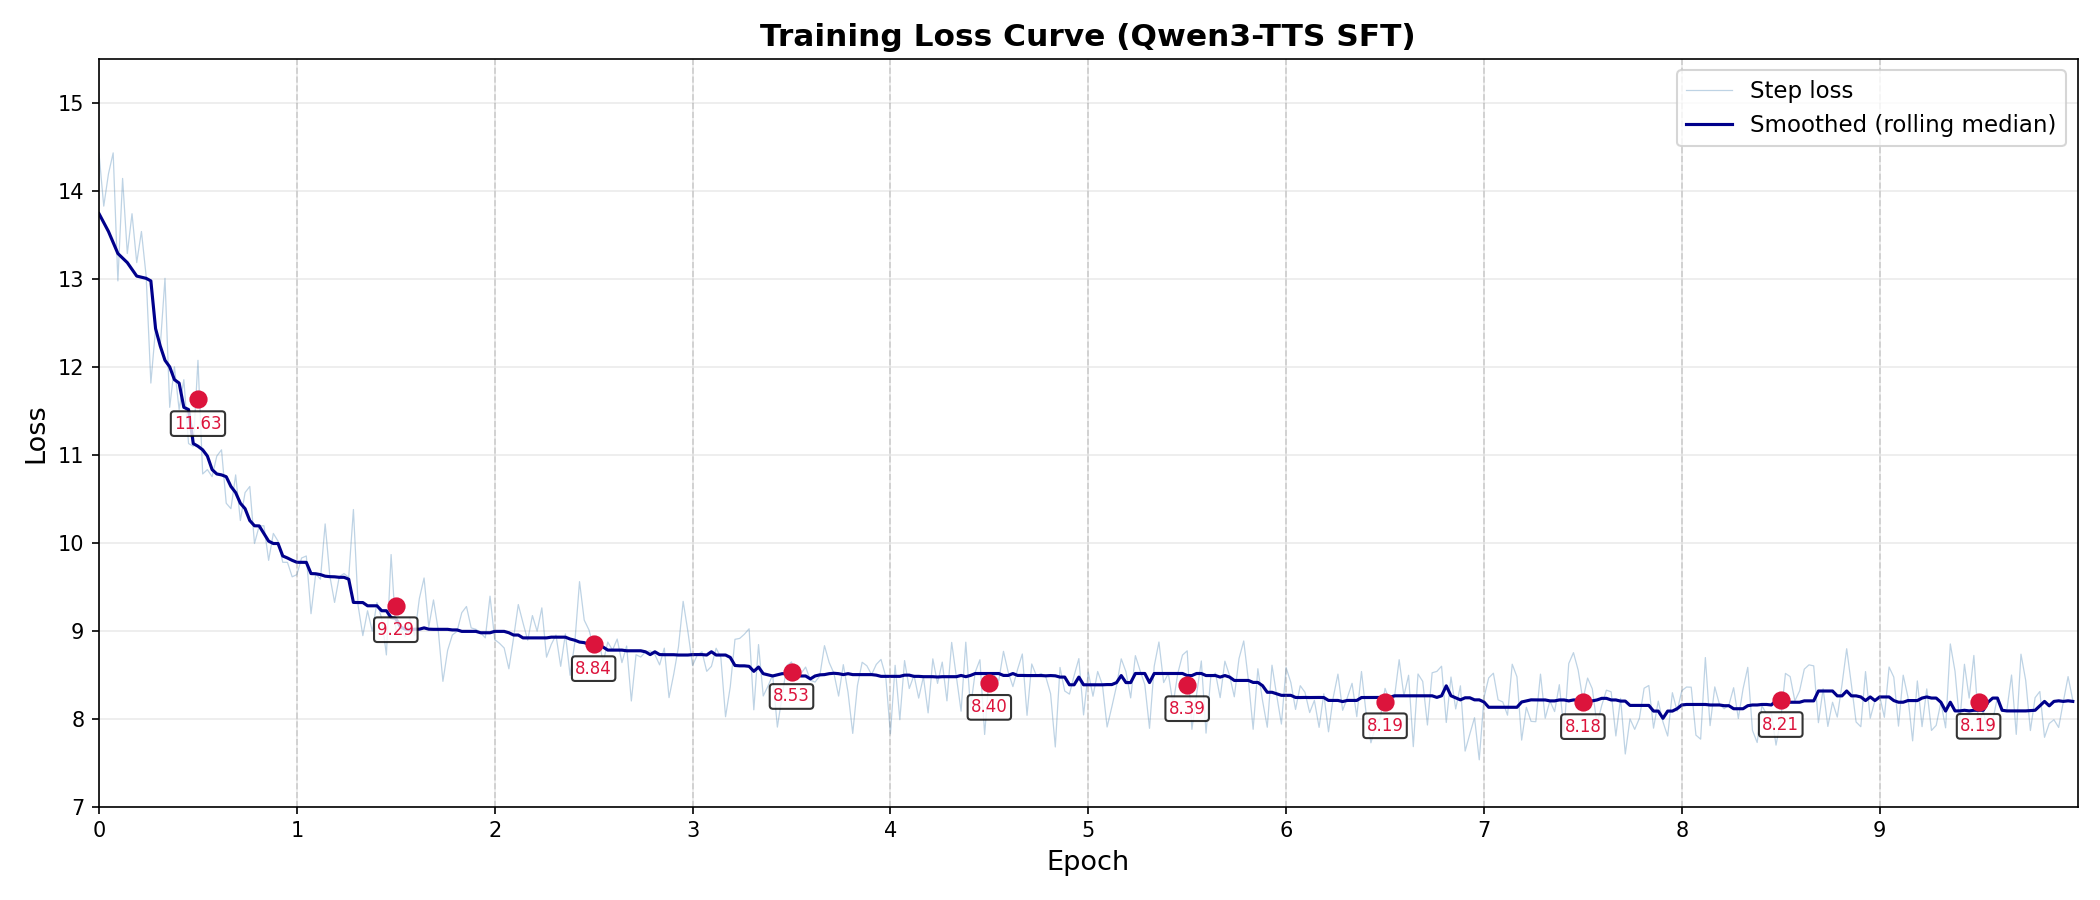
\includegraphics[keepaspectratio]{assets/lr=1e-6.png}}

}

\caption{LR=1e-6 训练 Loss 曲线}

\end{figure}%

从两张 Loss 曲线图可以直观看出差异：\texttt{lr=2e-5} 时 Loss 在 Epoch
0-1 期间剧烈震荡并快速下探，随后几乎不再下降；而 \texttt{lr=1e-6} 的
Loss 曲线呈现三个阶段------快速下降期（Epoch 0-2）→ 稳定下降期（Epoch
2-4）→ 收敛期（Epoch 4-9），训练过程更加健康可控。

\subsection{7.3 原因分析}\label{ux539fux56e0ux5206ux6790}

高学习率导致生成质量崩溃的根本原因与 Qwen3-TTS
的模型架构和微调方式密切相关：

\begin{enumerate}
\def\labelenumi{\arabic{enumi}.}
\item
  \textbf{全量微调的风险}：本项目使用的是全参数微调（Full
  Fine-Tuning），模型全部 1.7B
  参数都参与梯度更新。过大的学习率意味着每一步参数更新的幅度过大，极易''冲散''预训练权重中已编码的通用语音合成知识。
\item
  \textbf{Speaker Embedding 的特殊性}：微调过程中，speaker embedding
  是通过 speaker encoder 从训练数据中实时提取的（随后被注入到
  codec\_embedding 第 3000 位）。过大的参数更新会导致 speaker embedding
  与模型其他部分的''接口''失调------模型无法正确利用说话人特征来引导语音合成。
\item
  \textbf{Sub-talker 损失的敏感性}：总损失 = 主 loss + 0.3 × sub\_talker
  loss。Sub-talker 负责预测 15 层量化器的 codec tokens，其优化目标比主
  codec-0 预测更复杂。高学习率下两者的梯度冲突加剧，导致整体训练不稳定。
\item
  \textbf{小数据集的内在挑战}：训练数据仅 832
  条，远小于预训练语料规模。在数据量有限的情况下，需要更小的学习率来避免模型过度偏向训练集的有限分布。
\end{enumerate}

\subsection{7.4 经验教训}\label{ux7ecfux9a8cux6559ux8bad}

\begin{enumerate}
\def\labelenumi{\arabic{enumi}.}
\tightlist
\item
  \textbf{官方默认参数不可盲信}：官方示例的学习率 \texttt{2e-5}
  可能适用于大规模多说话人数据，但在单一说话人小数据集全量微调场景下可能完全不适用。
\item
  \textbf{Loss 不是唯一指标}：训练过程中应定期进行推理验证（如在每个
  epoch 结束后生成测试样本），而非仅依赖 Loss 数值判断训练效果。
\item
  \textbf{学习率需根据场景调整}：在全量微调大模型时，建议从小学习率（\texttt{1e-6}
  量级）起步，观察 Loss 下降趋势和生成效果后逐步调整。
\item
  \textbf{保留中间 checkpoint}：\texttt{sft\_12hz.py} 中每个 epoch
  保存一个 checkpoint
  的机制在此次问题排查中发挥了重要作用------通过对比不同 epoch
  的生成效果，能够清晰判断训练是否在正确的轨道上。
\end{enumerate}

\section{8. 总结}\label{sec-summary}

本项目基于 Qwen3-TTS-12Hz-1.7B-Base
大模型，通过全量微调成功实现了游戏角色「芙宁娜」的高质量语音克隆。以下从\textbf{完成工作}、\textbf{核心发现}和\textbf{未来方向}三个维度进行总结。

\subsection{8.1 完成工作}\label{ux5b8cux6210ux5de5ux4f5c}

{\def\LTcaptype{none} % do not increment counter
\begin{longtable}[]{@{}
  >{\raggedright\arraybackslash}p{(\linewidth - 4\tabcolsep) * \real{0.1500}}
  >{\raggedright\arraybackslash}p{(\linewidth - 4\tabcolsep) * \real{0.4000}}
  >{\raggedright\arraybackslash}p{(\linewidth - 4\tabcolsep) * \real{0.4500}}@{}}
\toprule\noalign{}
\begin{minipage}[b]{\linewidth}\raggedright
\#
\end{minipage} & \begin{minipage}[b]{\linewidth}\raggedright
工作项
\end{minipage} & \begin{minipage}[b]{\linewidth}\raggedright
关键结果
\end{minipage} \\
\midrule\noalign{}
\endhead
\bottomrule\noalign{}
\endlastfoot
1 & \textbf{数据处理} & 从 900+ 条原始音频中过滤出 832
条（3-15s），重采样至 24kHz，提取 12Hz codec tokens 用于训练 \\
2 & \textbf{全量微调} & 832 条数据 × 10 epoch，Loss 从 14.97 收敛至
2.38，完成 Base→CustomVoice 转换，speaker embedding 固化至
codec\_embedding{[}3000{]}，推理无需参考音频 \\
3 & \textbf{主观听感评测} & 4 组文本（中/英、短/长）× 3 个
checkpoint（Epoch 0/4/8），横向对比音色相似度、自然度和发音准确性 \\
4 & \textbf{量化指标评测} & 20 条样本 × 4 维度（Mel
MSE/Cosine、MFCC、STFT），Base vs SFT 对比实验。SFT 全面优于 Base：Mel
MSE ↓8.9\%，MFCC Cosine ↑5.4\% \\
5 & \textbf{问题排查} &
发现并解决了学习率过大导致生成崩溃的关键问题------默认 LR=2e-5
生成噪声，调整为 1e-6 后效果显著改善 \\
\end{longtable}
}

\subsection{8.2 核心发现}\label{ux6838ux5fc3ux53d1ux73b0}

\begin{enumerate}
\def\labelenumi{\arabic{enumi}.}
\item
  \textbf{学习率是微调成功的第一要素}：在全量微调 1.7B 大模型 +
  小数据集（832 条）的场景下，官方默认学习率 \texttt{2e-5}
  完全不适用，会导致模型遗忘预训练知识、生成纯噪声。降低至 \texttt{1e-6}
  是本次实验成功的转折点。这一发现提醒我们：\textbf{大模型微调的默认参数不可盲信，必须根据具体场景验证}。
\item
  \textbf{Loss 下降速度与生成质量并非正相关}：LR=2e-5 时 Loss
  下降极快，但生成效果反而最差；LR=1e-6 时 Loss
  平缓下降，生成质量却持续提升。在 TTS 微调中，\textbf{Loss
  值仅反映训练集上的 token 预测精度，无法替代实际听力评测}。
\item
  \textbf{量化指标有效验证了微调效果}：自建的 4 维评测管线（Mel MSE、Mel
  Cosine、MFCC Cosine、STFT Cosine）能够客观区分 Base 和 SFT
  模型的差异。其中 MFCC
  余弦相似度提升最为显著（+5.4\%），因其侧重音色特征，与微调目标高度吻合------验证了评测指标的合理性和微调的有效性。
\item
  \textbf{主观+客观双轨验证体系是可靠的质量保障}：主观听感测试给出了训练趋势的定性判断（音色随
  Epoch 增强、Epoch 8+
  可能过拟合），量化指标则提供了精确的数值支撑（各项指标变化百分比），两者互为补充，共同构成完整的评测闭环。
\end{enumerate}

\subsection{8.3
未来改进方向}\label{ux672aux6765ux6539ux8fdbux65b9ux5411}

{\def\LTcaptype{none} % do not increment counter
\begin{longtable}[]{@{}
  >{\raggedright\arraybackslash}p{(\linewidth - 2\tabcolsep) * \real{0.5000}}
  >{\raggedright\arraybackslash}p{(\linewidth - 2\tabcolsep) * \real{0.5000}}@{}}
\toprule\noalign{}
\begin{minipage}[b]{\linewidth}\raggedright
方向
\end{minipage} & \begin{minipage}[b]{\linewidth}\raggedright
说明
\end{minipage} \\
\midrule\noalign{}
\endhead
\bottomrule\noalign{}
\endlastfoot
\textbf{数据多样性扩充} &
增加不同情感、语速、语境的语音数据，提升模型表达能力和泛化性 \\
\textbf{Instruct 情感控制} &
在训练中加入情感/风格指令，实现多语气控制（开心、悲伤、愤怒等） \\
\textbf{超参数系统调优} & 对 learning rate、sub-talker loss 权重、batch
size 等关键参数进行系统搜索 \\
\textbf{更完善的客观评测} & 引入 MOS 评分、Speaker Embedding Cosine
Similarity、WER/CER 等指标 \\
\textbf{参数高效微调} & 探索
LoRA/QLoRA，在保持音色效果的同时大幅降低训练算力成本 \\
\end{longtable}
}

\section{9. 部署与使用}\label{sec-deploy}

\subsection{9.1 环境配置}\label{ux73afux5883ux914dux7f6e}

\subsubsection{安装依赖}\label{ux5b89ux88c5ux4f9dux8d56}

\begin{Shaded}
\begin{Highlighting}[]
\CommentTok{\# 安装 qwen{-}tts 核心包}
\ExtensionTok{pip}\NormalTok{ install qwen{-}tts}

\CommentTok{\# 安装推理所需依赖}
\ExtensionTok{pip}\NormalTok{ install torch transformers accelerate}
\ExtensionTok{pip}\NormalTok{ install flash{-}attn }\AttributeTok{{-}{-}no{-}build{-}isolation}
\ExtensionTok{pip}\NormalTok{ install gradio soundfile librosa}
\end{Highlighting}
\end{Shaded}

\subsubsection{下载模型}\label{ux4e0bux8f7dux6a21ux578b}

下载模型将其复制到 \texttt{finetuning/output/} 目录下：

\subsection{9.2 使用}\label{ux4f7fux7528}

下载 best\_model，配置好环境后将模型存放到 \texttt{finetuning/output/}
目录下，运行下面代码即可打开 Web 页面:

\begin{Shaded}
\begin{Highlighting}[]
\NormalTok{qwen}\OperatorTok{{-}}\NormalTok{tts}\OperatorTok{{-}}\NormalTok{demo finetuning}\OperatorTok{/}\NormalTok{output}\OperatorTok{/}\NormalTok{best\_model }\OperatorTok{\textbackslash{}}
  \OperatorTok{{-}{-}}\NormalTok{device cuda:}\DecValTok{0} \OperatorTok{\textbackslash{}}
  \OperatorTok{{-}{-}}\NormalTok{dtype bfloat16 }\OperatorTok{\textbackslash{}}
  \OperatorTok{{-}{-}}\NormalTok{ip }\FloatTok{0.0.0.0} \OperatorTok{\textbackslash{}}
  \OperatorTok{{-}{-}}\NormalTok{port }\DecValTok{8000}
\end{Highlighting}
\end{Shaded}

启动后，在浏览器中打开 \texttt{http://localhost:8000}
即可访问芙宁娜语音合成界面。在界面中：

\begin{figure}[H]

{\centering \pandocbounded{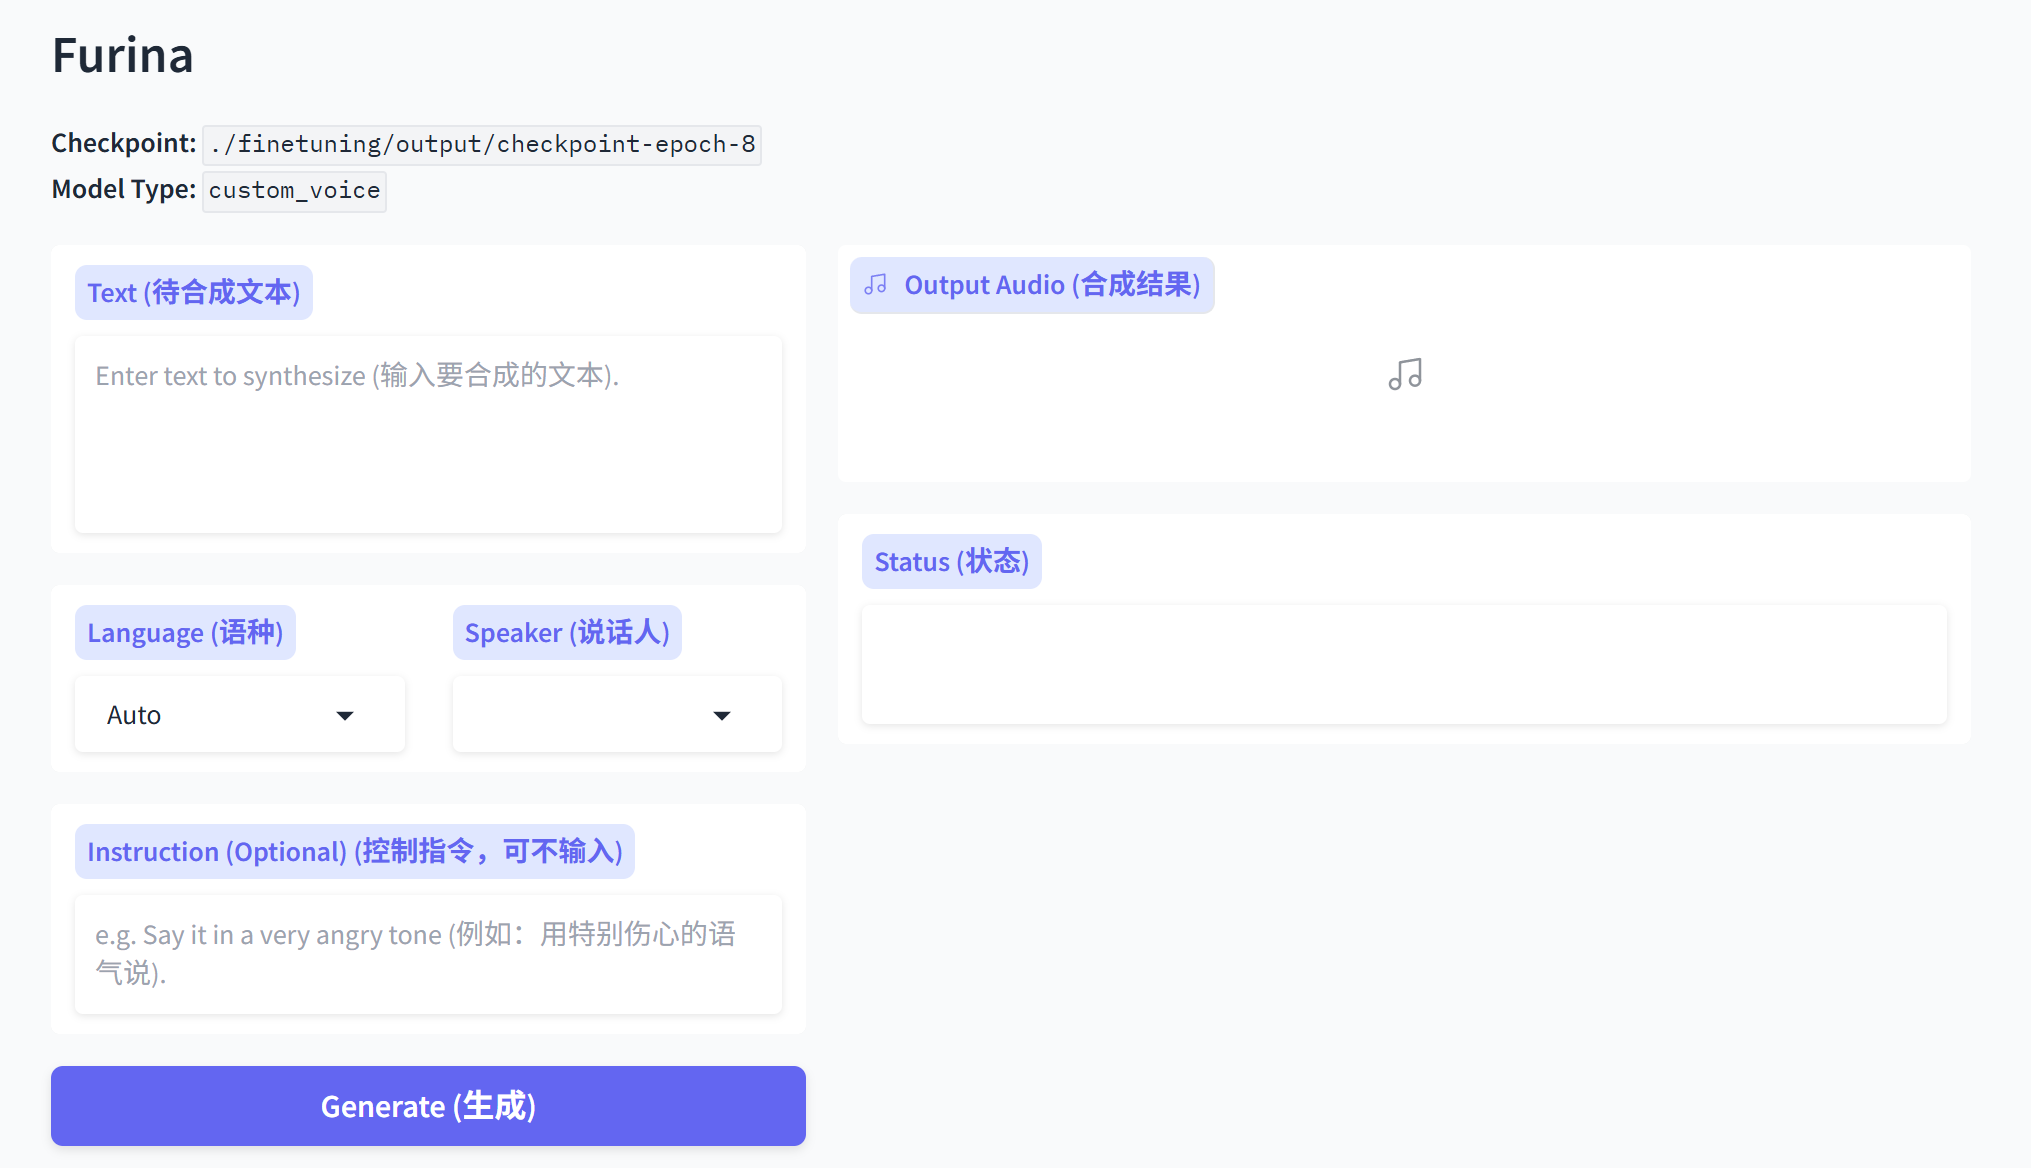
\includegraphics[keepaspectratio]{assets/web_demo.png}}

}

\caption{web\_demo}

\end{figure}%

\begin{enumerate}
\def\labelenumi{\arabic{enumi}.}
\tightlist
\item
  输入待合成的文本
\item
  选择语言（Auto / Chinese / English）
\item
  选择说话人 \textbf{furina}
\item
  可选：输入情感/风格控制指令（如「用开心的语气说」）
\item
  点击 \textbf{Generate（生成）} 按钮，即可获得合成语音
\end{enumerate}




\end{document}
